\subsection{Wav2Vec}

Wav2Vec~\cite{Schneider_Baevski_Collobert_Auli_2019} est un modèle de \gls{asr} proposé par Facebook AI.
Son architecture est composée d'un \gls{cnn} qui extrait des caractéristiques de l'entrée audio,
suivi d'un transformeur qui effectue le traitement séquentiel (voir Figure~\ref{fig.wav2vec}).


\begin{figure}[hbt]
    \centering
    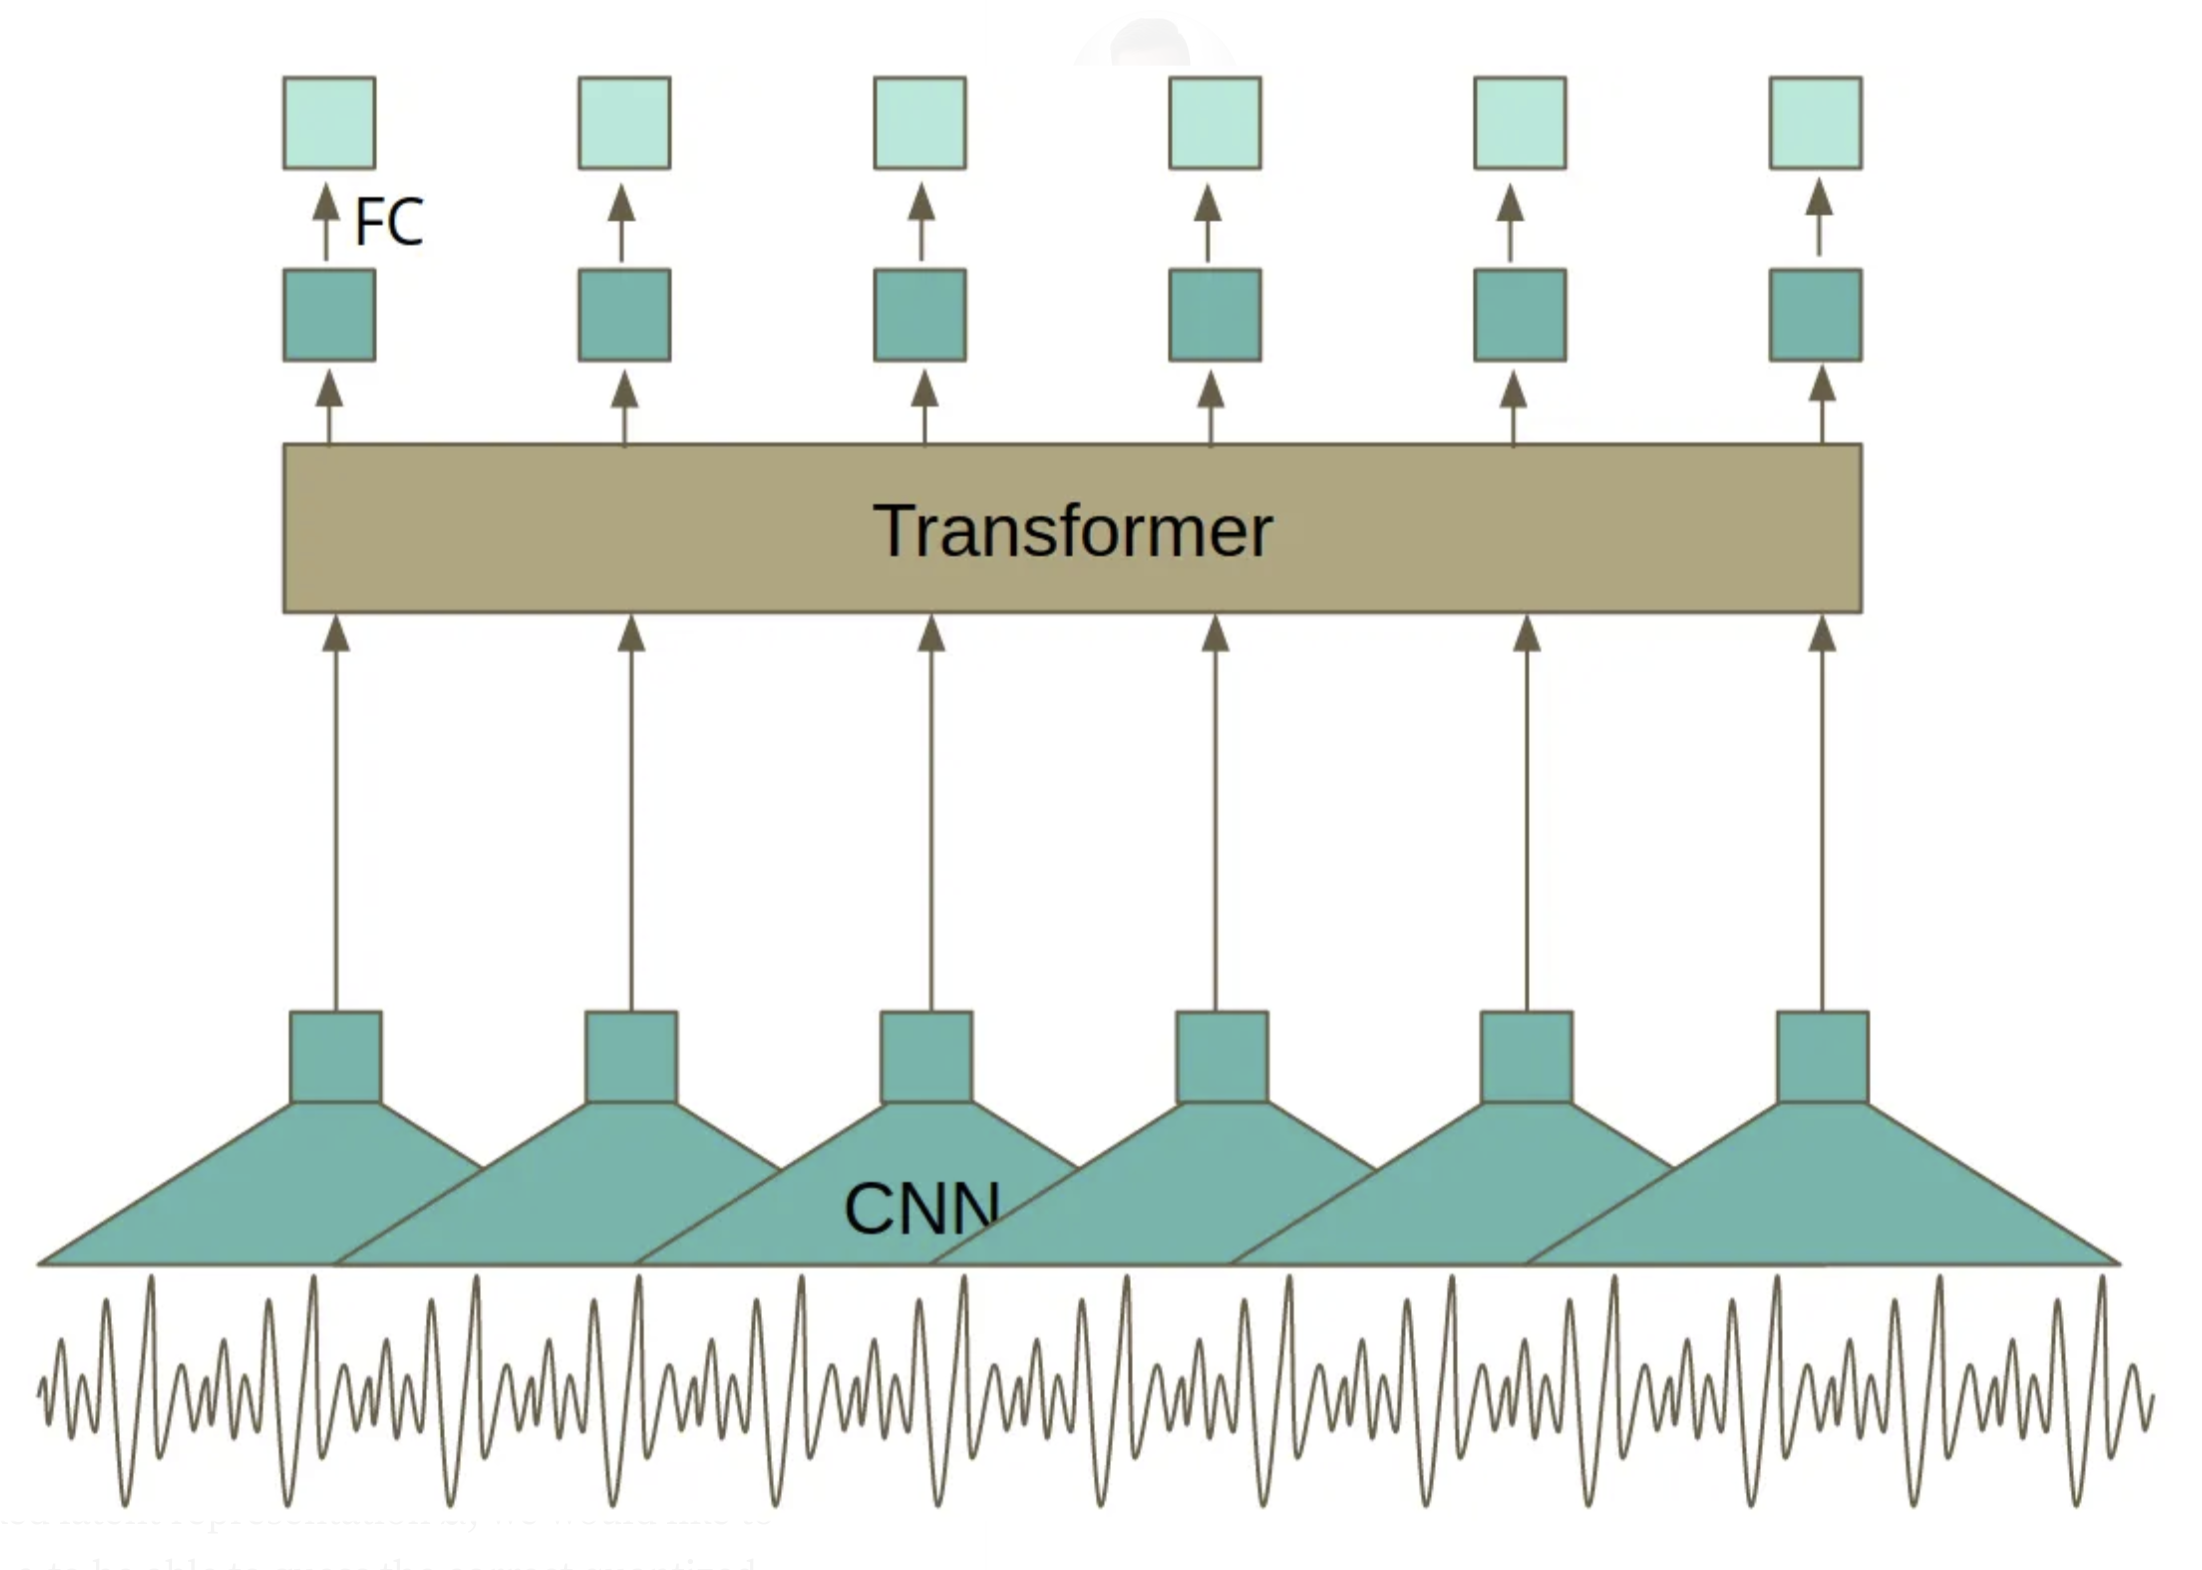
\includegraphics[width=.7\linewidth]{assets/images/wav2vec.png}
    \caption[Architecture de Wav2Vec.]{Architecture de Wav2Vec~\cite{Sus_2021}.}
    \label{fig.wav2vec}
\end{figure}